\documentclass[11]{article}
\usepackage{amsmath}
\usepackage[in]{fullpage}
\usepackage{tikz}
\usetikzlibrary{er}
\usetikzlibrary{positioning,shapes,shadows,arrows}
\newcommand{\HRule}{\rule{\linewidth}{0.3mm}}
\usepackage{multicol}
\usepackage{lipsum}% dummy text
\usepackage{tikz}
\usepackage{graphicx}
\numberwithin{equation}{section}

\def\checkmark{\tikz\fill[scale=0.4](0,.35) -- (.25,0) -- (1,.7) -- (.25,.15) -- cycle;} 
\setlength{\columnseprule}{0.4pt}
\begin{document}
\centerline{\Large \textsc{ \textbf{Home Management System}}} \smallskip
\centerline{\large \textsc{ \textbf{Project Proposal}}} \smallskip
\noindent\HRule \\
\ \\
\textbf{Description} \\
Home management portal to track home related activity such as expenses, grocery purchases, who is cooking next, whose turn is in cleaning trash using a combination of functions like expense manager, to do list, note taking utilities along with a instant messenger for member communication regarding the activity. \\
\ \\
\noindent \textbf{Users} \\
Each project(name for new profile) consists of groups. Group can be created by one or more individual members. The portal consists of three abstract activity.  \\
\ \\
\noindent \textbf{Activity} \\
Task, List and Expense. Task involves work which will consume time of the activity based on the type of work, example Trash cleaning or cooking. List is a way to specify items in a order or unordered form, grocery listing for next week or things to repair in house. Expense activity will involve the money component in it, grocery purchases, refueling vechile. One or more combination can be used to create groups. The groups will encompass members. The task alone group will be cooking turns. Expense activity will involve trips. List activity will involve. Below is the example of each.\\
\iffalse 
\begin{minipage}{0.32\textwidth}

\end{minipage}%
\hfill
\begin{minipage}{0.32\textwidth}
\begin{tabular}{|p{\textwidth}}

\end{tabular}
\end{minipage}%
\hfill
\begin{minipage}{0.32\textwidth}
\begin{tabular}{|p{\textwidth}}

\end{tabular}
\end{minipage}%

\begin{table}[h] % http://en.wikibooks.org/wiki/LaTeX/Tables
\begin{center}
\caption{Task }
	\begin{tabular}{| c | c |} % number of c's is the number of columns; options are r, l, c (that's a lowercase L). I also use a vertical pipe (|) for vertical lines in the table. This can get really confusing, since l (L) and | (pipe) look identical. Leave the pipes out of your default code.
	\hline
	Cooking & \checkmark \\  % put & between columns
	\hline
	Bob & \checkmark \\  % put & between columns
	\hline
		Ram & \checkmark \\  % put & between columns
	\hline
		Jay & \checkmark \\  % put & between columns
	\hline
		Diya & \checkmark \\  % put & between columns
	\hline
		Robert &  \\  % put & between columns
	\hline
		Linda &  \\  % put & between columns
	\hline
		John &  \\  % put & between columns
	\hline
	\end{tabular}
\end{center}
\end{table}


\begin{table}[h] % http://en.wikibooks.org/wiki/LaTeX/Tables
\begin{center}
\caption{Listing }
	\begin{tabular}{| c | c | c |} % number of c's is the number of columns; options are r, l, c (that's a lowercase L). I also use a vertical pipe (|) for vertical lines in the table. This can get really confusing, since l (L) and | (pipe) look identical. Leave the pipes out of your default code.
	\hline
	Cooking & Qty & \checkmark \\  % put & between columns
	\hline
	Rice & 10 kg & \checkmark \\  % put & between columns
	\hline
		Wheat Flour & 10 kg &  \\  % put & between columns
	\hline
		Tortilla & 10 pc & \\  % put & between columns
	\hline
		Milk & 3 Gallons & \\  % put & between columns
	\hline
		Eggs &  18 & \\  % put & between columns
	\hline
	\end{tabular}
\end{center}
\end{table}

\begin{table}[h] % http://en.wikibooks.org/wiki/LaTeX/Tables
\begin{center}
\caption{Expense }
	\begin{tabular}{| l | l | c |} % number of c's is the number of columns; options are r, l, c (that's a lowercase L). I also use a vertical pipe (|) for vertical lines in the table. This can get really confusing, since l (L) and | (pipe) look identical. Leave the pipes out of your default code.
	\hline
	Item & Cost & Paid by \\  % put & between columns
	\hline
	Rice & \$20 & Ram \\  % put & between columns
	\hline
		Wheat Flour & \$20 & Diya \\  % put & between columns
	\hline
		Tortilla & \$5 & John \\  % put & between columns
	\hline
		Milk & \$2.5 & \\  % put & between columns
	\hline
		Eggs &  \$4 & \\  % put & between columns
	\hline
	\end{tabular}
\end{center}
\end{table}
\fi
\ \\
\noindent \textbf{Scope} \\
Each users in the given project will have equal access. The groups can be created by members. Members can create new groups, add, delete or modify items. \\
\ \\
\noindent \textbf{Tables} \\
Login(\underline{username},password) \\
Members(\underline{member\_id},username,member\_name,email,phone) \\
Groups(\underline{group\_id},group\_name) \\
Member\_groups(\underline{member\_group\_id},group\_id,member\_id,member\_value) \\
Expenses(\underline{transaction\_id},group\_id,item,cost,expenses\_shared\_with) \\
Notes(\underline{note\_id},group\_id,list,status,pin\_to) \\
Tasks(\underline{task\_id},group\_id,task,status) \\
Messages(\underline{message\_id},to\_id,from\_id,message,time) \\
Schedules(\underline{schedule\_id},schedule\_activity,start\_date,schedule\_interval,iterations) \\
\ \\
\noindent \textbf{Table description} \\
\begin{enumerate}
\item[Login] Contains data for user credential verification.
\item[Members] Will hold all the member details.
\item[Groups] Members form a group which involve in certain activity. Expenses, Lists and Tasks uses this group as a reference to specific member activity.
\item[Member\_groups] This table reduces the redundancy of using both \emph{group\_id} and \emph{member\_id} in each activities(Expenses, Lists, Tasks) and as well as messages instead \emph{member\_group\_id} is used in it's place. \emph{member\_value} column is assigned unique value to a member within a group which enables to identify if only few member in that group involved in the group or all. For example, If a purchase is made and it should be shared between 3 members in a 5 member group. \emph{member\_value} column will help in identifying these three members out of 5 and expenses will be shared among only these 3.member\_value column contains value in powers of 2 to identify which member in the group is involved. For example, group containing 5 members. Consider a,b,c,d,e are 5 members relatively assigned as a as 1st member, b as second member $\cdots$ . 
\begin{align*}
\textit{member\_value}&=\displaystyle\sum_{i=1}^{n}2^{(i-1)}*x_i\\
\end{align*}
\begin{align*}
x_i =
  \begin{cases}
    1       & \quad \text{if } i^\text{th} \text{ is involved in activity}\\
    0  & \quad \text{if } i^\text{th} \text{ is not involved in activity}\\
  \end{cases} \\
\end{align*}
For the example,
\begin{align*}
\textit{only member a is involve}&=2^0*1+2^1*0+2^2*0+2^3*0+2^3*0=1\\
\textit{only member a and e is involve}&=2^0*1+2^1*0+2^2*0+2^3*0+2^3*1=1+16=17\\
\textit{only member a,c and e is involve}&=2^0*1+2^1*0+2^2*1+2^3*0+2^3*1=1+4+16=21\\
\textit{all members are involved}&=2^0*1+2^1*1+2^2*1+2^3*1+2^3*1=1+2+4+8+16=31\\
\end{align*}
This table needs both SQL and NoSQL database implementation to accommodate the Message table.
\item[Expenses] Activity involving expenses. \emph{expenses\_shared\_with column} references \emph{Member\_groups(member\_value)} to identify whether the expenses is of individual or whole group or few members in a group.
\item[Notes,Tasks] Activity involving Lists and Tasks. \emph{Shared\_with column} refers to who is a group this tasks is assigned to. Absence of pin\_to refers to tasks completed by that member.
\item[Messages] Message can be attached to any activity, group or individual based on \emph{to\_id}(sender of message by an individual) and \emph{from\_id}(reciever of the message to group or individual or selected members in a group for an activity). The given relation is given for a SQL database which will be translated to NoSQL database upon implementation.
\item[Schedules] Attaching the scheduling event to the activity(Expense,Notes,Task) or to a Group. Scheduling can be one time or recurring at a constant interval. \emph{interval} signifies the time gap between two activity. \emph{iterations} specifies number of times this activity should be repeated.\\
\end{enumerate}
\noindent \textbf{Entity Relationship Diagram} \\
\begin{figure}[h]
     \centering
          \label{ocpic}
                \includegraphics*[angle=360,origin=c,width=.6\linewidth]{ocp2}
\end{figure}
\iffalse \tikzstyle{every attribute} = [top color=white, node distance=2.5cm]
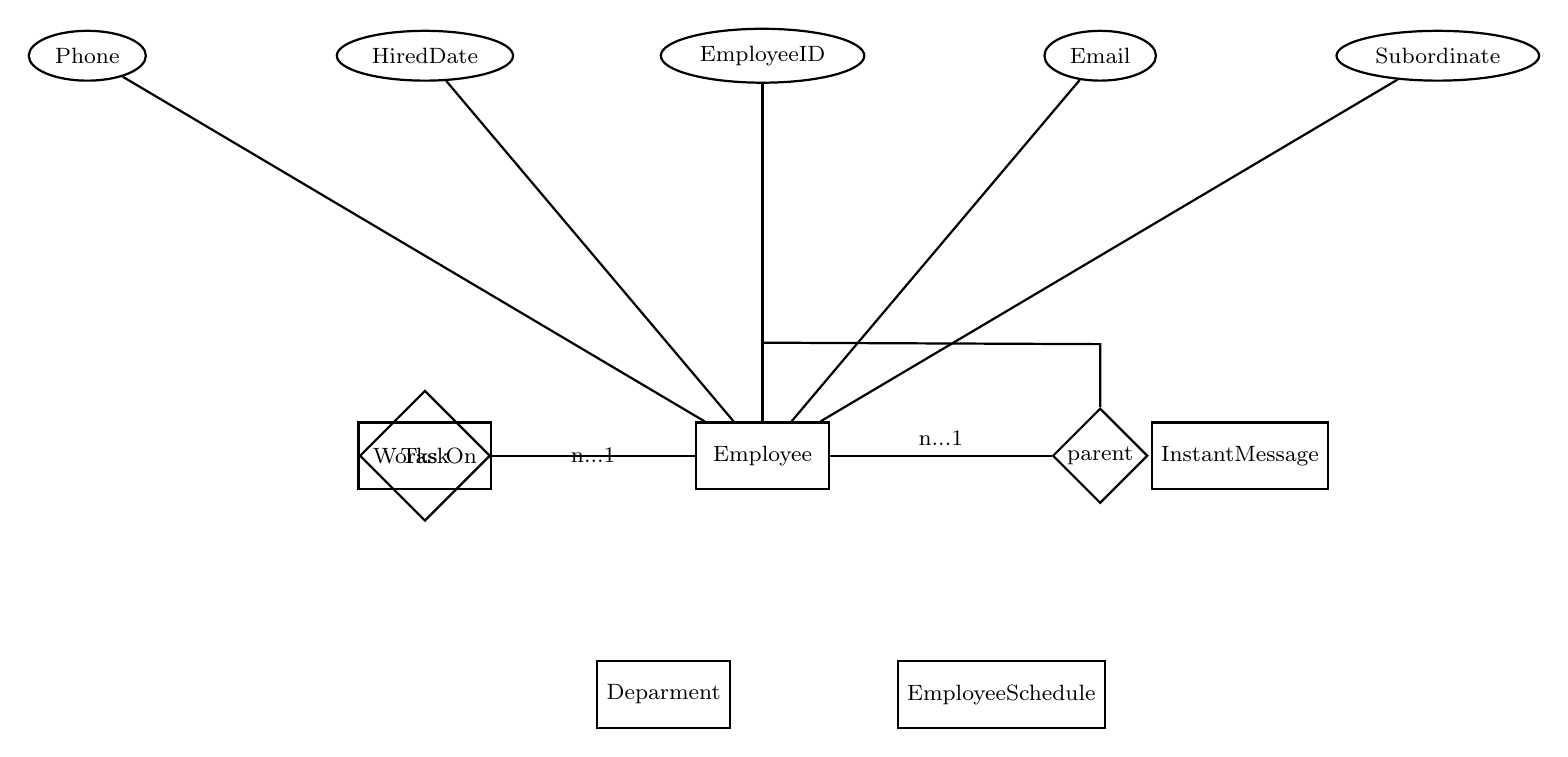
\begin{tikzpicture}[>=open triangle 90, thick,every node/.style={font=\footnotesize}, node distance = 12.2em]
\node[entity](Employee){Employee};
\node[attribute] (eid) [above=of Employee] {EmployeeID} edge (Employee);
\node[attribute] (hdate) [left of=eid] {HiredDate} edge (Employee);
\node[attribute] (email) [right of=eid] {Email} edge (Employee);
\node[attribute] (phone) [left of=hdate] {Phone} edge (Employee);
\node[attribute] (subordinate) [right of=email] {Subordinate} edge (Employee);

\node[entity](Task)[left of =Employee]{Task};

\node[entity](Deparment)[below right of =Task]{Deparment};

\node[entity](EmployeeSchedule)[right of =Deparment]{EmployeeSchedule};

\node[entity](InstantMessage)[above right of =EmployeeSchedule]{InstantMessage};

\node[relationship] (pageparent) [right of =Employee] {parent} edge node[above]{n...1} (Employee) edge (Employee);
\node[relationship] (EmployeeTask) [left of =Employee] {Works On} edge node {n...1} (Employee) edge (Task);
\coordinate[above= 1cm of Employee] (cpage);
\coordinate[above= 0.8cm of pageparent] (cpageparent);
\draw[-] (Employee)--(cpage)--(cpageparent)--(pageparent);
\end{tikzpicture}
\fi
\ \\
\noindent \textbf{Implementation} \\
Database implementation is using PostgreSQL and MongoDB(Messaging and member\_groups table alone). User interface is either using html/php or J2EE(JSP) or AngularJS. \\
\ \\
\noindent \textbf{Dataset} \\
For the project the personal available data is used having 7 years of personal expenses, trips, grocery bills. The available data is modified to suite to the project. Remaining data will be created. \\
\iffalse
\begin{table}[h]
\begin{center}
	\begin{tabular}{| c | c | c | c |}
	\hline
	\textbf{Timeline} & \textbf{Task} & \textbf{ETA}\footnote{Tentative Estimated Time of Accomplishment} & \textbf{Status} \\  % put & between columns
	\hline
	\begin{tabular}{@{}c@{}}Week 1 \\ ($5^{th}-11^{th}$ March)\end{tabular}  & \begin{tabular}{@{}c@{}}Users, Table(With sample data), Views, \\ Constraints, SQL queries to retrieve and load\end{tabular}  & 10 hrs & \\  % put & between columns
	\hline
	\begin{tabular}{@{}c@{}}Week 2 \\ ($12^{th}-18^{th}$ March)\end{tabular} & \begin{tabular}{@{}c@{}}Procedures, Functions, \\ Complete DB level implementation\end{tabular}  & 12 hrs &  \\  % put & between columns
	\hline
	\begin{tabular}{@{}c@{}}Week 3 \\ ($19^{th}-25^{th}$ March)\end{tabular} & \begin{tabular}{@{}c@{}}Front-end/UI Interface \\ (with known technology J2EE,JSP/PHP)\end{tabular} & 10 hrs &  \\  % put & between columns
	\hline
	\begin{tabular}{@{}c@{}}Week 4 \\ ($26^{th}$ March $-1^{th}$ April)\end{tabular} & Instant Messaging through MongoDB & 14 hrs & \\  % put & between columns
	\hline
	\begin{tabular}{@{}c@{}}Week 5 \\ ($9^{th}-15^{th}$ April)\end{tabular} & Front-end implementation using Angular JS & 15 hrs & \\  % put & between columns
	\hline
	\begin{tabular}{@{}c@{}}Week 6 \\ ($16^{th}-22^{nd}$ April)\end{tabular} & Front-end implementation using Angular JS & 15 hrs &  \\  % put & between columns
	\hline
	\begin{tabular}{@{}c@{}}Week 7 \\ ($23^{rd}-29^{th}$ April)\end{tabular} & \begin{tabular}{@{}c@{}}Performance, Security testing and \\ enhancement, Report\end{tabular}  & 10 hrs &  \\  % put & between columns
	\hline
	\begin{tabular}{@{}c@{}}Week 8 \\ ($23^{rd}-29^{th}$ April)\end{tabular}  & \begin{tabular}{@{}c@{}}Slide preparation and presentation \\ of project\end{tabular}  & 8 hrs &  \\  % put & between columns
	\hline
	\end{tabular}
\label{ }
\end{center}
\end{table}
\fi
\end{document}